\documentclass[fontsize=8pt, a4paper, landscape, fleqn]{scrartcl}

\usepackage[utf8]{inputenc}
\usepackage[english]{babel}
%\usepackage[standardsections]{scrhack}
%\usepackage[raggedright]{titlesec} %% Gives warnings
\usepackage{xcolor, sectsty}
\usepackage{algpseudocodex}
\usepackage{enumerate, enumitem, ulem, graphicx, multirow, comment}
\usepackage{listings}
\usepackage{wrapfig} 
\usepackage{titlesec}     % For customizing section titles
\usepackage{graphicx}     % Required for dimensions with \parbox

%Graph
\usepackage{tikz}
\usetikzlibrary{positioning}
\usetikzlibrary{trees}
\usepackage{pgfplots}

%Page reference
\usepackage{hyperref}
\usepackage{xparse,nameref}
\hypersetup{
    pdfborder={0 0 0}, % Add this line to remove the link border
}

%code layout
\definecolor{sec}{RGB}{40,56,71}
\definecolor{subsec}{RGB}{72,98,124}
\definecolor{subsubsec}{RGB}{102,141,178}
\definecolor{codegreen}{rgb}{0,0.6,0}
\definecolor{codegray}{rgb}{0.5,0.5,0.5}
\definecolor{codepurple}{rgb}{0.58,0,0.82}
\definecolor{backcolour}{RGB}{240,240,240}
\usepackage{tcolorbox}
\tcbuselibrary{minted, breakable}

% Define custom colors
\definecolor{sectioncolor}{RGB}{64, 64, 64}       % Dark Gray
\definecolor{subsectioncolor}{RGB}{70, 130, 180}  % Steel Blue

% Custom section and subsection commands with unified styling
\renewcommand{\section}[1]{%
    \noindent\colorbox{sectioncolor}{%
        \parbox{\dimexpr\columnwidth-2\fboxsep}{\color{white}\textbf{#1}}}%
    \vspace{0.5mm}% Optional spacing after the section
}

\renewcommand{\subsection}[1]{%
    \noindent\colorbox{subsectioncolor}{%
        \parbox{\dimexpr\columnwidth-2\fboxsep}{\color{white}\textbf{#1}}}%
    \vspace{0.5mm}% Optional spacing after the subsection
}

% Optional: Customize subsubsection or other title levels
\renewcommand{\subsubsection}[1]{%
    \noindent\textbf{\textit{\color{subsectioncolor}#1}}% Italic with subsection color
    \vspace{1mm}% Optional spacing after subsubsection
}
%Layout
\usepackage{multicol, geometry, titlesec, xcolor}
\geometry{margin=0.2cm}
%\titlespacing{\section}{0pt}{3pt}{1pt}
%\titlespacing{\subsection}{0pt}{3pt}{1pt}
%\titlespacing{\subsubsection}{0pt}{3pt}{1pt}
\parindent 0pt

%Remove numbering
\pagestyle{empty} 
%\pagenumbering{arabic}

\setlist[itemize]{leftmargin=2mm, itemsep=0mm} %{nosep}
\setlist[enumerate]{leftmargin=3mm, nosep} %{nosep}

\newlength{\breite}
\setlength{\breite}{0.5pt}
\setlength{\columnseprule}{\breite}

\usepackage{graphicx}

%Style code
\usepackage{minted}
\lstdefinestyle{mystyle}{
    backgroundcolor=\color{backcolour},
    commentstyle=\color{codegreen},
    keywordstyle=\color{blue},
    numberstyle=\tiny\color{codegray},
    stringstyle=\color{codepurple},
    basicstyle=\ttfamily,
    breakatwhitespace=false,
    breaklines=true,
    captionpos=b,
    keepspaces=true,
%    numbers=left,
    numbersep=5pt,
    showspaces=false,
    showstringspaces=false,
    showtabs=false,
    tabsize=2,
}
\lstset{style=mystyle}

%Mathematics
\usepackage{amsmath, amstext, amssymb, mathtools, esint, polynom}
\allowdisplaybreaks %Seitenumbruch in align-Umgebung erlauben

%Document file
\begin{document}

	\begin{multicols*}{3}[\raggedcolumns]
 
	\section{Git}
	\subsection{Configuration}
    First configure git by setting the name of the user for commits
    \begin{lstlisting}[language=C, breaklines]
    $ git config --global user.name "eth" \end{lstlisting}
    Then set the email address
    \begin{lstlisting}[language=C, breaklines]
    $ git config --global user.email "eth@ethz.ch" \end{lstlisting}
    
    \subsection{Starting project}
    \textbf{Initialize directory}
    \begin{lstlisting}[language=C, breaklines]
    $ git init [project name] \end{lstlisting}
    Then it's of upmost importance to \lstinline{add} and \lstinline{commit -m "..."}, otherwise git will not have a main branch and it will back the error \lstinline{fatal: not a valid object name: 'main'}.\\
    \textbf{Diff between edited and added}
    \begin{lstlisting}[language=C, breaklines]
    $ git diff \end{lstlisting}
    
    \textbf{Diff between added and committed}
    \begin{lstlisting}[language=C, breaklines]
    $ git diff --cached\end{lstlisting}
    
    \subsection{Branching}
    \textbf{Create a new branch}
    \begin{lstlisting}[language=C, breaklines]
    $ git branch [NAME] \end{lstlisting}
    
    \textbf{Show all branches} \lstinline{-a} .
    \begin{lstlisting}[language=C, breaklines]
    $ git branch [-a] \end{lstlisting}

    \textbf{Switch between branches}
    \begin{lstlisting}[language=C, breaklines]
    $ git checkout [NAME] \end{lstlisting}

    \textbf{Merging an external branch into the one that the user is currently in} 
    \begin{lstlisting}[language=C, breaklines]
    $ git merge [NAME] \end{lstlisting}
    
    \textbf{Delete a branch} 
    \lstinline{-d} and its name
    \begin{lstlisting}[language=C, breaklines]
    $ git branch -d [NAME] \end{lstlisting}
    
    \subsubsection{How to solve conflicts}
    Git will show the differences in the files of the local version compared to the one on the cloud. Then the user have to make literally merging the two version, while git will proceed to upload the merged version on the server. If get an error when pulling, you can set \lstinline{git pull --no-rebase} and then by checking with \lstinline{git status} you'll be able to see which files need to be merged. An useful command is \lstinline{git diff}, which shows the difference between the repository states.
    
	\section{Preprocessing / compiling / linking}
    \subsection{Preprocessing}
    Errors of missing files are detected at this stage.\\
    \textbf{List of useful commands for preprocessor macros:}
    \begin{itemize}
        \item \lstinline{#define ADD(A+B) A+B}
        \item \lstinline{#define f(x) std::sin(x)}
        \item \lstinline{#if __has_include(<format>)#include <format> #define HAS_FORMAT #else}
        \item \lstinline{#if defindef(ADD) && (YYY==1)}
        \item \lstinline{#undef f // Removes macro def.}
        \item \lstinline{#ifdef SYMBOL}
        \item \lstinline{#else}
        \item \lstinline{#endif // End macro def. at this point, useful with ifdef}
        \begin{itemize}
            \item example: \begin{lstlisting}[language=C, breaklines]
#ifdef DEBUG
...
#else 
...
#endif \end{lstlisting}
        Throught the shell is possible to define \lstinline{DEBUG} before compile time with \lstinline{-DDEBUG}.
        \end{itemize}
        \item \lstinline{#error MESSAGE_ERROR} shows the error if this macro is reached by the program.
    \end{itemize}

	\subsection{general linking process}
    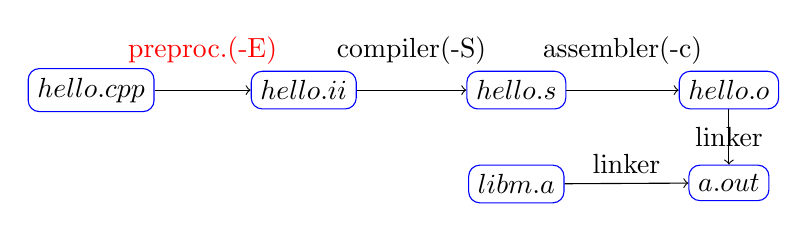
\begin{tikzpicture}[main/.style = {node distance=27mm, rectangle, draw=blue, rounded corners}] 
        \node[main] (1) {$hello.cpp$}; 
        \node[main] (2) [right of=1] {$hello.ii$}; 
        \node[main] (3) [right of=2] {$hello.s$}; 
        \node[main] (4) [right of=3] {$hello.o$}; 
        \node[main] (5) [below=7mm of 3] {$libm.a$}; % Adjust the vertical spacing here
        \node[main] (6) [below=7mm of 4] {$a.out$}; % Adjust the vertical spacing here
        \draw[->] (1) -- node[midway, above, yshift=2mm] {\textcolor{red}{preproc.(-E)}} (2);
        \draw[->] (2) -- node[midway, above, yshift=2mm] {compiler(-S) } (3);
        \draw[->] (3) -- node[midway, above, yshift=2mm] {assembler(-c)} (4);
        \draw[->] (4) -- node[midway] {linker} (6);
        \draw[->] (5) -- node[midway, above] {linker} (6);
    \end{tikzpicture}
    \textcolor{red}{Only non sys. dependent}

	\subsection{command line linking}
    In case of multiple file, the linking works by creating first all the \lstinline{.o} files:

    \begin{lstlisting}[language=C++, breaklines]
    $ c++ -c square.cpp
    $ c++ -c main.cpp
    $ c++ main.o square.o -o square
    // name output executable is square \end{lstlisting}

    \section{Header}
    \subsection{Guards}
    Guards are set in the header as follow, but it's also possible to use \lstinline{pragma once}, instead of declaring the header.
    % First, it's possible to use \lstinline{pragma once}, instead of declaring the header.
    % Usually guards are set in the header as:
    \begin{lstlisting}[language=C++, breaklines]
    #ifndef EXAMPLE_H 
    #define EXAMPLE_H
    ...
    #endif /*SIMPSON_H*/ \end{lstlisting}
    \textcolor{red}{Missing include guards: May cause compilation errors (e.g., redefinitions).}\\
    \section{Libraries}
    \subsection{Static library} 
    File extension: \lstinline{lib* .a} (a stands for archive) and these are \textbf{copied into} the \textbf{executable}.
    Steps to create: first compile file and create object \lstinline{.o}, after we require to create an archive with \lstinline{ar} as

    \begin{lstlisting}[language=C++, breaklines]
    $ ar -crs libNAME.a NAME.o \end{lstlisting}

    with \textcolor{red}{\lstinline{lib}}\lstinline{NAME}\textcolor{red}{\lstinline{.a}}.
        
    \subsection{shared library}
    Here is a difference between a static library in the compiling of the \lstinline{lib* .cpp}. We need to specify \textcolor{red}{\lstinline{l-fPIC}} and set in the shell

    \begin{lstlisting}[language=C++, breaklines]
    $ c++ -fPIC -c NAME.cpp \end{lstlisting}
    
    File extension: \lstinline{lib* .so} (shared object), everything \textbf{loaded into} the \textbf{memory} (RAM).
    Steps to create:  like before but we change the extension, \lstinline{-shared} add \lstinline{-fPIC}
    
    \begin{lstlisting}[language=C++, breaklines]
    $ ar -shared -fPIC -o libNAME.so NAME.o \end{lstlisting}

    and as before we must set \textcolor{red}{\lstinline{lib}}\lstinline{NAME}\textcolor{red}{\lstinline{.so}}.

    \subsection{Link with executable}
    Example with \textcolor{red}{\lstinline{Ilib}} and \textcolor{red}{\lstinline{Llib}}, which \textcolor{red}{\lstinline{-I}} specifies the directory of the header and \textcolor{red}{\lstinline{-L}} the directory of the library:
    \begin{lstlisting}[language=C++, breaklines, emph={-Ilib, -Llib}, emphstyle={\color{red}}]
    $ c++ -c -Ilib main.cpp 
    $ c++ -o EXAMPLE main.o -Llib -lEXAMPLE \end{lstlisting}
    
   \subsubsection{Link with subfolders}
One useful example is at \lstinline{ex02/simpson}. In the main makefile, we need to specify the folder of the library:
\begin{lstlisting}[language=make, breaklines, emph={src}, emphstyle={\color{red}}]
CXX = c++
LDFLAGS = -Lsrc
LDLIBS = -lex
main: main.cpp src/libex.a
    $(CXX) -o $@ $< $(LDFLAGS) $(LDLIBS)
\end{lstlisting}
\subsubsection{Linking against Libary in Makefile}
\begin{lstlisting}[language=make, breaklines, emph={src}, emphstyle={\color{red}}]
CXX = c++
.PHONY: all clean
all: main
simpson.o: simpson.cpp simpson.hpp
    ${CXX} -c $<
libsimpson.a: simpson.o
    ar -crs $@  $<
main.o: main.cpp
    ${CXX} -c $< 
main: main.o libsimpson.a
    ${CXX} -o $@ $< -L. -lsimpson
.PHONY: clean
clean:
    rm *.o


\end{lstlisting}
    
    \subsection{Documentation}
     Ex. at weed02a, pg.27. A library must be documented with the following points:
    \begin{multicols}{2}
    \begin{itemize}
        \item \textbf{Synopsis}: of functions, types, variables declared
        \item \textbf{Semantics}: Purpose of the function
        \item Preconditions
        \item Postconditions
        \item Dependencies
        \item Exception guarantees: ...
        \item References/additional material
    \end{itemize}
    \end{multicols}
    \subsection{Checklist for Documenting Functions and Templates}

\begin{itemize}
    \item \textbf{Synopsis:} 
    \begin{itemize}
        \item What does the function do?
        \item Briefly describe its purpose and use case.
    \end{itemize}

    \item \textbf{Semantics:}
    \begin{itemize}
        \item Describe the high-level behavior of the function.
        \item Include any special computational details.
    \end{itemize}

    \item \textbf{Requirements:}
    \begin{itemize}
        \item \textbf{Template Parameters:} Clearly specify constraints for each parameter:
        \begin{itemize}
            \item For \texttt{F}: Must be callable, accepting a single argument convertible from \texttt{T}, and returning a value convertible to \texttt{T}.
            \item For \texttt{T}: Must support arithmetic operations (\texttt{+}, \texttt{-}, \texttt{*}, \texttt{/}) and be \texttt{CopyConstructible} and \texttt{Assignable}.
        \end{itemize}
        \item \textbf{Supported Operations:} Explicitly define the operations that \texttt{F} and \texttt{T} must support, such as:
        \begin{itemize}
            \item \texttt{operator+}, \texttt{operator-}, etc., for arithmetic on \texttt{T}.
            \item Callable operations (\texttt{F(x)}), where \texttt{x} is within the interval \([a, b]\).
        \end{itemize}
    \end{itemize}

    \item \textbf{Preconditions:}
    \begin{itemize}
        \item List what must be true before calling the function (e.g., non-null pointers, valid ranges).
    \end{itemize}

    \item \textbf{Postconditions:}
    \begin{itemize}
        \item Specify what is guaranteed after the function completes if preconditions are met.
        \item Document changes to arguments or global state.
    \end{itemize}

    \item \textbf{Dependencies:}
    \begin{itemize}
        \item Mention external libraries, helper functions, or type traits the function relies on.
    \end{itemize}

    \item \textbf{Exception Guarantees:}
    \begin{itemize}
        \item Specify if the function is \texttt{noexcept} or what exceptions it might throw.
        \item Detail the level of exception safety (basic, strong, or no guarantee).
    \end{itemize}

    \item \textbf{References:}
    \begin{itemize}
        \item Link to related material, such as documentation or textbooks.
    \end{itemize}
\end{itemize}
    \section{Make}
    
    Basic example (full example at \colorbox{blue!7}{\autoref{sec:makefile}}):
    \begin{lstlisting}[language=make, breaklines]
    square.o: square.cpp square.hpp
        c++ -c square.cpp
    main.o: main.cpp square.hpp
        c++ -c main.cpp
    square: main.o square.o
        c++ -o square main.o square.o \end{lstlisting}
    \textbf{If I run make $\Rightarrow$ only builds square.o $\Rightarrow$ make square}
    \subsection{Automatic variables}
    With automatic variables the example becomes:
    \begin{lstlisting}[language=make, breaklines]
    square.o: square.cpp square.hpp
        c++ -c $<
        # <: insert file name of first prerequisite
    main.o: main.cpp square.hpp
        c++ -c $<
    square: main.o square.o
        c++ -o $@ $^
        # @: file name of target, 
        # ^: names all prerequisites \end{lstlisting}

    \subsection{Predefined variables variables}
    List of possible commands:

    \begin{multicols}{2}
    \begin{itemize}
        \item \lstinline{CC} compiler \lstinline{cc}
        \item \lstinline{CXX} compiler \lstinline{g++}
        \item \lstinline{RM} remove as \lstinline{rm -f}
        \item \lstinline{CFLAGS} set flags for \lstinline{C}
        \item \lstinline{CXXFLAGS} set flags for \lstinline{C++}
        \item \lstinline{LDFLAGS} Flags when linking
        \item \lstinline{LDLIBS} Library flags
    \end{itemize}
    \end{multicols}

    We can modify again the previous example as

    \begin{lstlisting}[language=make, breaklines]
    square.o: square.cpp square.hpp
        ${CXX} ${CXXFLAGS} -c $<
    main.o: main.cpp square.hpp
        ${CXX} ${CXXFLAGS} -c $<        
    square: main.o square.o
        ${CXX} ${CXXFLAGS} -o $@ $^

    .PHONY: clean
    clean: ${RM} -v *.o square \end{lstlisting}

    To the predefined variables can be given a specific variable like \lstinline{CXX = c++} (use \lstinline{+= for multiples})or we can set a file \lstinline{config.mk} and reference it at the beginning of the makefile to include specific settings (automatic ignored if doesn't exits).

    \begin{lstlisting}[language=make, breaklines]
    include config.mk

    .PHONY: all clean
    all: square
    
    square.o: square.cpp square.hpp
        ${CXX} ${CXXFLAGS} -c $<
    main.o: main.cpp square.hpp
        ${CXX} ${CXXFLAGS} -c $<        
    square: main.o square.o
        ${CXX} ${CXXFLAGS} -o $@ $^

    .PHONY clean
    clean: ${RM} -v *.o square
    \end{lstlisting}
    
	\section{CMake}
 
	\subsection{Setup}
    Example at \colorbox{red!7}{\autoref{sec:cmake}}. First create the folder named \textcolor{blue}{\lstinline{build}}, file \textcolor{blue}{\lstinline{CMakeLists.txt}} and then type

    \begin{lstlisting}[language=C, breaklines]   
$ cmake .. // there must be a CMakeLists.txt 
           // file in the directory
           // containing the whole project \end{lstlisting}

    to create the folder in which the executables will be stored. Then to compile all the files just type \lstinline{make} in the directory \lstinline{build}. Other important commands:
    
    \begin{multicols}{2}
    \begin{itemize}
        \item \lstinline{$ make NAME}: build NAME
        \item \lstinline{$ make clean}: clean build
        \item \lstinline{$ make install}: install dependencies
    \end{itemize}
    \end{multicols}

    \subsubsection{Static library} 
    To include a static library, we need to add the library at the beginning of the \lstinline{CMakeLists.txt} as follow

    \begin{lstlisting}[language=make, breaklines, emph={STATIC}, emphstyle={\color{red}}]
    add_library(squareLib STATIC square.cpp)
    ...\end{lstlisting}

    \subsubsection{Shared library}
    For a shared, we just need to change static to shared.
    
    \begin{lstlisting}[language=make, breaklines, emph={SHARED}, emphstyle={\color{red}}]
    add_library(squareLib SHARED square.cpp)
    ...\end{lstlisting}
    \section{Classes}
    Def: Collection of Members ( Functions, Data, Types)
    
    \subsection{Operator Overloading}
Syntax: type \textcolor{green}{operator} \textcolor{blue}{OP} (arguments) $\{ *...body...*\}$, need to use the \textcolor{red}{friend} keyword to overload operator as Non-member fkts if private or protected members of the class need to be accessed 

\subsubsection{Increment/Decrement}
\begin{lstlisting}[language=C++]
// Prefix Increment
MyClass& operator++(); 
// Returns a reference to the updated object.
// Postfix Increment
MyClass operator++(int);
// Returns a copy of the object before increment.
\end{lstlisting}

\subsubsection{Arithmetic Operators}
\begin{lstlisting}[language=C++]
// Addition
MyClass operator+(const MyClass& other) const;
// Returns a copy of the result.
// Compound Addition
MyClass& operator+=(const MyClass& other);
// Returns a reference to the modified object.
\end{lstlisting}

\subsubsection{Comparison Operators}
\begin{lstlisting}[language=C++]
// Equality/Inequality
bool operator==(const MyClass& other) const;
bool operator!=(const MyClass& other) const;
// Returns a boolean value.
// Relational Operators
bool operator<(const MyClass& other) const;
// Returns a boolean value.
\end{lstlisting}

\subsubsection{Stream Operators}
\textcolor{red}{Always return os}
\begin{lstlisting}[language=C++]
// Output Stream
friend std::ostream& operator<<(std::ostream& os, const MyClass& obj);
// Returns a reference to the output stream for chaining.
// Input Stream
friend std::istream& operator>>(std::istream& is, MyClass& obj);
// Returns a reference to the input stream for chaining.
\end{lstlisting}

\subsubsection{Subscript Operator}
\begin{lstlisting}[language=C++]
// Non-const Subscript
MyClass& operator[](std::size_t index);
// Returns a reference to the element (modifiable).
// Const Subscript
const MyClass& operator[](std::size_t index) const;
// Returns a const reference to the element (read-only).
\end{lstlisting}

\subsubsection{Pointer-like Operators}
\begin{lstlisting}[language=C++]
// Dereference
MyClass& operator*();
// Returns a reference to the object pointed to.
// Member Access
MyClass* operator->();
// Returns a pointer to the object.
\end{lstlisting}

\subsubsection{Assignment Operator}
\begin{lstlisting}[language=C++]
// Assignment
MyClass& operator=(const MyClass& other);
// Returns a reference to the modified object.
\end{lstlisting}

\subsubsection{Unary Operators}
\begin{lstlisting}[language=C++]
// Unary Minus
MyClass operator-() const;
// Returns a copy of the negated object.
// Logical NOT
bool operator!() const;
// Returns a boolean value.
\end{lstlisting}

\subsection{Member function/Non-member functions}
\textbf{\textcolor{black}{Member function:} \texttt{A::operator@()} or \textcolor{black}{Non-member function:} \texttt{operator@(A)}} (if applicable).

\textbf{\textcolor{green}{Unary Operators} (\texttt{@a}) (\texttt{+}, \texttt{-}, \texttt{*}, \texttt{\&}, \texttt{!}, \texttt{\~}, \texttt{++}, \texttt{--})}:  
Can be both member and non-member functions.

\textbf{\textcolor{green}{Binary Operators} (\texttt{a@b}) (\texttt{+}, \texttt{-}, \texttt{*}, \texttt{/}, \texttt{\%}, \texttt{<<}, \texttt{>>}, \texttt{\&\&}, \texttt{||}, \texttt{<}, \texttt{>}, etc.)}:  
Can be both member and non-member functions.

\textbf{\textcolor{red}{Compound Assignment Operators} (\texttt{a@=b}) (\texttt{=},\texttt{+=}, \texttt{-=}, \texttt{*=}, \texttt{/=}, \texttt{\%=}, etc.)}:  
Must be member functions (\texttt{A::operator@=(B)}).

\textbf{\textcolor{red}{Special Operators} (a(b, c...)}{ (Function Call), ), a$\rightarrow$b (Pointer Access), (TYPE)a (Type Conversion)}:

Must be a member function 

\textbf{Member functions}: when the left operand must be a class object (e.g., \texttt{a->b}, \texttt{a(b)}).

\textbf{Non-member functions}: when the operator requires symmetry or involves conversions on the left operand (e.g., \texttt{a + b}).
\begin{lstlisting}[language=C++, breaklines]
// Member function implementation
class A {
public:
    A operator+(const A& other) const {
        return A(); // Example logic
    }
};

// Non-member function implementation
A operator+(const A& a, const A& b) {
    return A(); // Example logic
}
\end{lstlisting}

\noindent CPP Reference: $cpp/language/operators$

    \subsection{Public}
    \subsubsection{Constructor} 
    Use \textcolor{red}{explicit} to shield from missus
    \begin{lstlisting}[language=C++, breaklines]
Resource() : data_(nullptr), size_(0) {};
explicit Resource(size_t size) : data_(new int[size]), size_(size) {};
\end{lstlisting}
\textcolor{red}{Allocate an array of ints with new int[size]}

\subsubsection{Destructor} 
    \begin{lstlisting}[language=C++, breaklines]
~Resource() {
    delete[] data_; // Use delete[] for arrays
    data_ = nullptr; // Optional but good practice
}\end{lstlisting}
\textcolor{red}{You need delete[] data for arrays}

    \subsubsection{Copy constructor} 
    Creates a new  \textcolor{red}{deep} copy of the object. \textcolor{red}{Allocating new memory.}
    \begin{lstlisting}[language=C++, breaklines]
Resource(const Resource& other)
    : data_(new int[other.size_]), size_(other.size_) {
    for (size_t i = 0; i < size_; ++i) {
        data_[i] = other.data_[i];
    }
}\end{lstlisting}

    \subsubsection{Copy Assignment} 
    Deep copies an existing object into another. This pointer is returned to allow chained assignments. 
    Need to handle self assignment.
    \textcolor{red}{Use swap instead of delete }
    \begin{lstlisting}[language=C++, breaklines]
Resource& operator=(const Resource& other) {
    if (this != &other) { // Handle self-assignment
        delete[] data_;
        data_ = new int[other.size_];
        size_ = other.size_;
        for (size_t i = 0; i < size_; ++i) {
            data_[i] = other.data_[i];
        }
    }
    return *this;
}
Resource& operator=(const Resource& other) {
    Resource temp(other); // Create a copy of `other`
    std::swap(data_, temp.data_); //(#include <utility>)
    std::swap(size_, temp.size_);
    return *this;
}\end{lstlisting}
    \subsubsection{Move constructor}
    Instead of duplicating the data, ownership of the resources is moved to the new object.
Adding noexcept ensures that this move constructor works efficiently with STL containers
    \begin{lstlisting}[language=C++, breaklines]
Resource(Resource&& other) noexcept : data_(other.data_), size_(other.size_) {
    other.data_ = nullptr;
    other.size_ = 0;
}\end{lstlisting}
    
    \subsubsection{Move assignment}
    Moves a temporary object into another object. Need to handle self assignment. \textcolor{red}{Clears the state of the rhs (other) after transferring ownership of its resources}
    \begin{lstlisting}[language=C++, breaklines]
Resource& operator=(Resource&& other) noexcept {
    if (this != &other) {
        delete[] data_; // Free current resources
        data_ = other.data_;
        size_ = other.size_;
        other.data_ = nullptr;
        other.size_ = 0;
    }
    return *this;
    }
    \end{lstlisting}
    \subsubsection{Namespaces and Functions}
    When describing a function from the \lstinline{.hpp} in the \lstinline{.cpp} file, we need to set up
    \begin{lstlisting}[language=C++, breaklines]
namespace example {
    // Definition of static data members
    type_t Example::HPP_FUNC(){
        // Define return value
    };
} // Close namespace \end{lstlisting}
\subsection{Tips for Simple Array Implementation}

\begin{itemize}
    \item \textbf{Make Constructors and Conversion Operators Explicit:}
    Avoid implicit conversions by marking constructors and conversion operators as \texttt{explicit}. This ensures conversions are intentional and prevents unintended behavior.

    \item \textbf{Use \texttt{swap} to Implement Copy Assignment:}
    Instead of deleting and reassigning resources in a copy assignment operator, use the \texttt{swap} idiom. It simplifies resource management and ensures exception safety.

    \item \textbf{Use Compound Arithmetic Operators:}
    Implement binary arithmetic operators (e.g., \texttt{+}, \texttt{-}) using compound arithmetic operators (e.g., \texttt{+=}, \texttt{-=}). This avoids redundancy and improves maintainability.

\end{itemize}
    \subsection{Private}
    Logically, this is the opposite of private, and in a class everything is private by default.
    
    \subsection{Protected} 
    Protected is very similar to \lstinline{private}, only it applies also to derived types, thus should be used only for member functions and not data. Non member functions can't access this section.

    \subsection{Static Members}
Static members are shared across all objects of a class. If modified, the change is reflected in all instances. Static functions can only access static member variables, not non-static ones. Static data members must be \textbf{declared} in the class and \textbf{defined} (and optionally initialized) outside the class, typically in a .cpp file. For important const static members, initialization can be done in the class if they are constant expressions (cannot be modif.).
    \subsection{const member funtions}
    Rule: Make all fkt const (between () and $\{\}$) and then decide weather they need to change the object. 
    \subsection{Mutable members}
    In case we have a constant object, we can still change its value through \lstinline{mutable}, one example is to modify a value called by a const function.

    \begin{lstlisting}[language=C++, breaklines, emph={mutable}, emphstyle={\color{red}}]   
class A {
    public:
        int func() const;
    private:
        mutable int cnt_;
};
int A::func() const {
    cnt_++; // OK!
return 42;} \end{lstlisting}

    \subsection{Function objects} 
     Used if we want to use an object (class, struct) like a function, or we cant pass the fnkt. directly (e.g. function takes two arguments, we only need one. For that we overload 
     \lstinline{operator()(variables...)}. 

    \begin{lstlisting}[language=C++, breaklines, emph={operator}, emphstyle={\color{red}}]   
class Func {
    public:
        Func(double l) : lambda(l) {}
        double operator()(double x) {
           return exp(-lambda*x);
        }
    private:
        const double lambda;
    };
    Func f(3.5);
    Integrate(f, 0., 1., 1000); \end{lstlisting}
\subsection{Lambda Expressions (C++11)}
\begin{itemize}
    \item \texttt{[]} - Capture nothing.
    \item \texttt{[$\&$]} - Capture all referenced variables by reference.
    \item \texttt{[=]} - Capture all referenced variables by copy.
    \item \texttt{[=, \&foo]} - Capture all by copy, but \texttt{foo} by reference.
    \item \texttt{[bar]} - Capture only \texttt{bar} by copy.
    \item \texttt{[this]} - Capture the \texttt{this} pointer.
\end{itemize}

\begin{lstlisting}[language=C++, breaklines, emph={operator}, emphstyle={\color{red}}]
// Example: Capturing 'lambda' by value
lambda = -3.5;
auto f = [lambda](double x) { return std::exp(-lambda * x); };

// Using the lambda function
integrate(f, 0., 1., 1000);
\end{lstlisting}
Here [lambda]` captures `lambda` by value,modify the capture list as needed (e.g., `[$\&$]` for reference).
    \section{Generic programming}
    \subsection{Templates} 
    Set before the call of a function.

    \begin{lstlisting}[language=C++, breaklines, emph={template, Function}, emphstyle={\color{red}}]
template <typename Function>
std::vector<double> Integrator(Function f)
{...}\end{lstlisting}


    Then, when calling the function, we need to specify the type for the template as \lstinline{function_name<type>}.

    \subsection{Class Templates} 
Allow defining classes that work with generic types. By specifying a \texttt{template} before type is determined at the time of instantiation. 
\begin{lstlisting}[language=C++, breaklines, emph={T}, emphstyle={\color{red}}]
template <typename T>
class Point {
public:
    using coord_t = T;
    coord_t abs(); // Declaration
    ...
};
// Definition of member function outside the class (We need the typename here)
template <typename T>
typename Point<T>::coord_t Point<T>::abs() {
    ...
}
// Creating instances with specific types
Point<float> pf;    // float coordinates
Point<double> pd;   // double coordinates
\end{lstlisting}
    \subsection{Metaprogramming}
    We start with a simple example in which we return the type instead of a value such that we calculate values at compile time:

    \begin{lstlisting}[language=C++, breaklines, emph={using}, emphstyle={\color{red}}]   
template <typename T>
struct ReturnType {
    using type = T;}; \end{lstlisting}

    \subsection{Type traits} 
    Example at \colorbox{orange!7}{\autoref{sec:traits}}.
    With type traits we can set a similar overloading operator but for structures such that a function can still work with different kind of values.
    
    \begin{lstlisting}[language=C++, breaklines, emph={typedef}, emphstyle={\color{red}}]   
// Definition of the struct min_type
template <typename T, typename U> struct min_type { };

// Case in which we have same types. Notices the typename for T
template <typename T> struct min_type<T, T> { typedef float type; };

// Case in which we have two distinct types
template <> struct min_type<float, int> { typedef float type; };
 
min(1,2.3f); // Result will be min_type<int, float>::type = float \end{lstlisting}
    
    With traits we need to specify the type of the output in case we have two different types comparing with each other. In case we are working in a function and we need to specify the type of the template, we can use \lstinline{::type}:

    \begin{lstlisting}[language=C++, breaklines, emph={using, T,type}, emphstyle={\color{red}}]   
template <typename T>
typename average_type<T>::type average(std::vector<T> const& v) {
    using D = typename average_type<F>::type;
    D sum = 0;
    // ...
} \end{lstlisting}
\lstinline{average_type<T>::type}defines the return type of the function. The \lstinline{typename} keyword is required because \lstinline{average_type<T>} is a dependent type, and the compiler needs to treat type as a type name.
\textcolor{red}{\lstinline{typename} T type is the same as using type = T}
    \section{Exceptions}
    \subsection{Error handling} 
    Errors can be resolved through exceptions, and we can start with the example:

\begin{lstlisting}[language=C++, breaklines]
#include <stdexcept>

if( index >= size() )
   throw std::range_error("index"); \end{lstlisting}

    And it's possible to use the following commands:

    \begin{itemize}
            \item Logic errors:
        \begin{itemize}          \item \lstinline{domain_error}: value outside domain
            \item \lstinline{invalid_argument}: argument is invalid
        \end{itemize}
            \item Runtime errors: 
        \begin{itemize}
            \item \lstinline{range_error}: invaliv calue occurred
            \item \lstinline{overflow_error}: value too big
        \end{itemize}
    \end{itemize}

    And these errors can be avoided with \lstinline{try} and \lstinline{catch}. Example:

    \begin{lstlisting}[language=C++, breaklines]
int main() {
  try {
    ... // Function that returns a throw
  }  catch (std::exception& e) {
    std::cerr << "Error: " << e.what();
    // catch exceptions derived from std::exception
  } catch (...) {
   ...
   // catch all other exceptions
   // and/or throw error
   }
} \end{lstlisting}

    It's \textcolor{red}{important} that the destructor must not fail to clean, or if a catch can't deal with the exception then it's possible to re-throw.

    Example at \colorbox{purple!7}{\autoref{sec:exceptions}}.
    
	\section{Testing}

    Example at \colorbox{yellow!7}{\autoref{sec:test}}.
    First, in the \lstinline{CMakeLists.txt} in the main and the test folder, there must be \lstinline{enable_testing()}. After preparing all the correct \lstinline{CMakeLists.txt}, we can use the commands \lstinline{make test} or \lstinline{make all test} to build up the files. Just remember it might be possible that this will build mainly the test files, and not the main. 
    \textcolor{red}{Important:} in the files which we will put the test, we need to set an \lstinline{if} case in which inside there will be a throw, without \lstinline{catch}. Otherwise the test will always return true.

	\section{Date and time}
    To calculate the time, we need the following libraries
    \begin{itemize}
        \item \lstinline{<ctime>}: normal date and time
        \item \lstinline{<chrono>}: precision measurement
    \end{itemize}
    \begin{itemize}
    \item \texttt{(b - a).count()}: Directly retrieves the raw duration in the clock's \textbf{native time unit} (e.g., nanoseconds or milliseconds), without converting it to another unit.
    \item \texttt{std::chrono::duration<T>(b - a).count()}:Converts the duration to a \textbf{specific unit} (e.g., seconds with \texttt{std::chrono::duration<double>}) before retrieving its value.
\end{itemize}
    An example for a timer is located under \begin{lstlisting}[language=C++]
#include <iostream>
#include <chrono>
#include <thread>

int main() {
    auto start = std::chrono::high_resolution_clock::now();  // Start time
    std::this_thread::sleep_for(std::chrono::seconds(2));    // Simulate work
    auto end = std::chrono::high_resolution_clock::now();    // End time
    auto duration = std::chrono::duration<double>(end - start).count(); // Duration in seconds
    std::cout << "Elapsed time: " << duration << " seconds." << std::endl;
    return 0;
}
\end{lstlisting}
 
	% \section{Monte Carlo}
 %    Used for multiple dimension integration, which with Simpson would be too slow.
 %    INSERT EXAMPLE WTH EXPLANATIONS
 
	\section{Random numbers}
    Also in this case is possible to use a library, which is called \lstinline{random} or \textcolor{gray}{Boost}. But it's in general not possible to have a perfect randomisation on a finite machine.
	First is always necessary to set a seed:

 \begin{lstlisting}[language=C++, breaklines]
#include <random>
...
// default random engine
std::default_random_engine e;
e.seed(42); // set seed ONLY ONCE 
// Uniform
std::uniform_int_distribution<int> dist1(a,b);
std::uniform_real_distribution<double> dist2(lambda);
// Exponential
std::exponential_distribution<double> dist3(lambda);
//Normal
std::normal_distribution<double> dist4(mu, sigma);
double random_number = dis2(e);
std::random_device rd;
std::mt19937 gen(rd());
std::uniform_real_distribution<> dis(0.0, 1.0);
double random_number = dis(gen);\end{lstlisting}

    \section{Algorithms and data structures}
	\subsection{Complexity}
    
    \subsection{STL}
    
    This is the Standard Template Library which one example is \lstinline{<utility>}:
        \begin{lstlisting}[language=C++, breaklines, emph={typedef}, emphstyle={\color{red}}]
#include <utility>;
template <class T1, class T2>
class pair {
    public:
        T1 first;
        T2 second;
        pair(const T1& f, const T2& s) 
            : first(f), second(s) {}    }; \end{lstlisting}

    \subsection{Data structures}
    \begin{multicols}{3}
    \begin{itemize}
        \item \lstinline{Arrays}
        \begin{itemize}
            \item \lstinline{array}
            %\item \lstinline{valarray}
            \item \lstinline{vector}
            \item \lstinline{deque}
        \end{itemize}
        \item \lstinline{Linked lists}
        \begin{itemize}
            \item \lstinline{list}
        \end{itemize}
        \item \lstinline{Trees}
        \begin{itemize}
            \item \lstinline{map}
            \item \lstinline{set}
            \item \lstinline{multimap}
            \item \lstinline{multiset}
        \end{itemize}
        \item \lstinline{Queues and stacks}
        \begin{itemize}
            \item \lstinline{queue}
            \item \lstinline{priority_queue}
            \item \lstinline{stack}
        \end{itemize}
    \end{itemize}
    \end{multicols}
    
	\subsubsection{Binary tree}
    \begin{multicols}{2}
    \begin{itemize}
        \item Number of nodes: $N=2^n-1$
        \item Access times: $\mathcal{O}(ln(N))$
        \item Possible data structures:  
        \begin{itemize}
            \item \lstinline{set}  
            \item \lstinline{multiset}
            \item \lstinline{map}  
        \end{itemize}
    \end{itemize}
    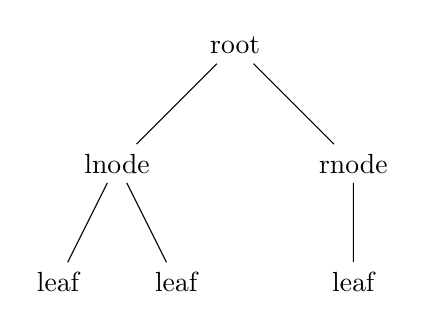
\begin{tikzpicture}[level distance=1.5cm,
        level 1/.style={sibling distance=3cm},
        level 2/.style={sibling distance=1.5cm}]
        \node {root}
        child {node {lnode}
          child {node {leaf}}
          child {node {leaf}}
        }
        child {node {rnode}
        child {node {leaf}}
        };
    \end{tikzpicture}
    \end{multicols}

	\subsection{Iterators}
    Example of iterator for Linked List:
    \begin{lstlisting}[language=C++, breaklines, emph={typedef}, emphstyle={\color{red}}]
template <typename T>
struct node_iterator {
  node<T>* p;
  node_iterator(node<T>* q) : p(q) {}
  node_iterator<T>& operator++() { p=p->next; return *this; }
  T* operator->() { return &(p->value); }
  T& operator*() { return p->value; }
  bool operator!=(const node_iterator<T>& x) { return p!=x.p; }
  // more operators missing
};
template<typename T>
struct slist {
  using iterator = node_iterator<T>;
  slist() : first(nullptr) {}
  iterator begin() { return iterator(first); }
  iterator end() { return iterator(nullptr); }
  // ...
};
for (slist<int>::iterator p=l.begin();
     p!=l.end();
++p) {
} std::cout << *p << " "; \end{lstlisting}

	\subsection{Containers and sequences}
	\subsection{Generic algorithms}
    Reference to the \lstinline{cpp reference} website under \href{https://en.cppreference.com/w/cpp/algorithm}{https://en.cppreference.com/w/cpp/algorithm} for more algorithms and \href{https://en.cppreference.com/w/cpp/iterator}{https://en.cppreference.com/w/cpp/iterator}.
	\subsection{Algorithms overview}
     Here there is a list of some algorithms presented in class, set with the header \lstinline{<algorithm>} (see week07)
     Use \lstinline{std::mem_fn} to wrap class functions. They cannot take an argument, must be part of the object in the container, or use \texttt{[this](int x) \{ return this->mem\_fnkt(x); \}} (See \lstinline{ex07/penna/src/population.cpp})

    \begin{multicols}{3}
    \begin{itemize}
        \item \lstinline{for_each}  
        \item \lstinline{find, find_if}
        \item \lstinline{count, count_if}  
        \item \lstinline{search}  
        \item \lstinline{transform}  
        \item \lstinline{copy, copy_backward}  
        \item \lstinline{swap}  
        \item \lstinline{replace, replace_if}  
        \item \lstinline{remove, remove_if}  
        \item \lstinline{reverse, reverse_copy}  
        \item \lstinline{sort}  
        \item \lstinline{lower_bound, upper_bound}  
        \item \lstinline{next_permutation}  
        \item \lstinline{set_union}  
        \item \lstinline{min, max}  
        \item \lstinline{min_element, max_element}  
        \item \lstinline{unique}  
    \end{itemize}
    \end{multicols}
	\section{Inheritance} 
\begin{lstlisting}[language=C++, breaklines]
class Derived : public Base { ... } ;\end{lstlisting}
    a new class called \lstinline{Base} set on the properties of \lstinline{Derived}.
    To see more examples on this, check \lstinline{demo/week08} in the repository 
	\subsection{Regarding classes}
    It's important to remember that protected variables set in the super class share the same value in each derived class.
\begin{lstlisting}[language=C++, breaklines]
class Polygon {
  public:
    void set_values(double a, double b) { // ... }
  protected:
    double width_, height_;
};
class Rectangle: public Polygon {
  public:
    double area() {
      return width_*height_;
    } };\end{lstlisting}
    The derived class inherits all members of the base class except Constructors and destructors, Assignment operators Friends, Private members
    \subsubsection{Constructor and destructor}
    Constructors cannot be virtual, but in the subclasses we need to specify the constructor based on the declaration of the superclass as follow:
\begin{lstlisting}[language=C++, breaklines, emph={Mother}, emphstyle={\color{red}}]
class Son : public Mother {
    public:
        Son(int a) : Mother(a) {};\end{lstlisting}

	\section{Polymorphism} 
    \lstinline{virtual} 
allows a class to define a function in the base class that can be overridden in derived classes with different implementations. This ensures that the correct function is called when using a \textbf{pointer or reference to the base class}, enabling runtime polymorphism.
\begin{lstlisting}[language=C++, breaklines, emph={typedef}, emphstyle={\color{red}}]
class Polygon {
    public:
        ...
        virtual double area() = 0;
        protected:
            double width_, height_; };
    
class rectangle : public Polygon{
    public:
        // Includes area (by default) 
        // width_, height_ can be used here
}; 
Triangle tri;
tri.set_values(4., 5.);
std::cout << "Triangle area: " << tri.area();
Polygon* poly;
poly = &tri; 
std::cout << "Triangle area: " << poly->area() << '\n';
// BECAUSE WE USED VIRTUAL IN ABC RIGHT AREA IS CALLED
\end{lstlisting}

    This can be used also for variables and functions.

\subsection{Abstract Base classes, see week08}
provide a mechanism for polymorphism by allowing functions to operate on pointers or references to the base class without knowing the derived class at compile time.
\textcolor{red}{ABCs cannot be instantiated alone but they can have constructors}
use override keyword to redefine a function from the ABC in the derived class
make destructors virtual to avoid leaks

\subsubsection{Runtime Polymorphism:}
\begin{itemize}
    \item Uses \textbf{virtual functions}.
    \item Decision at \textbf{runtime}.
    \item Works for objects derived from a \textbf{common base class}.
    \item Only \textbf{one function} created for the base class (saves space).
    \item Virtual function calls require \textbf{vtable lookup} (slower).
    \item Extension possible by defining new \textbf{derived classes}.
    \item Best for \textbf{application frameworks}, \textbf{user interfaces}, and large functions.
\end{itemize}
\subsubsection{Compile time polymorphism}
\begin{itemize}
    \item Uses \textbf{templates}.
    \item Decision at \textbf{compile-time}.
    \item Works for objects with \textbf{required members} (concepts).
    \item A \textbf{new function} created for each class (uses more space).
    \item No virtual calls; \textbf{inlined} for better performance.
    \item Extension requires definitions of all functions.
    \item Best for \textbf{low-level constructs}, small, fast functions, and \textbf{generic algorithms}.
\end{itemize}

    \section{Hardware}
    \subsection{Properties}
    
    \subsubsection{Assembly}
    Important properties:
    \begin{itemize}
        \item one to one translation from machine code to readable
        \item non-portable on other machines
    \end{itemize}
    
    \subsubsection{Machine code}
    The CPU performs action by reading the memory in form of machine code.
    % \begin{itemize}
    %     \item \lstinline{one to one translation from machine code to readable}  
    %     \item \lstinline{non-portable on other machines}
    % \end{itemize}
    
    \subsection{Pipelining}
    Method to speed up execution with parallelism (ILP).
    
    \subsubsection{Branch prediction}
    In few words, this can predict how a pipeline run and if the prediction is correct, then there is a gain in time. Otherwise abort pipeline and start right branch.

    \subsubsection{Parallelisation}
    There are two methods for memory access with parallelisation:
    \begin{multicols}{2}
    \begin{itemize}
        \item Shared memory architecture $\rightarrow$ multiple CPUs share \textbf{one} memory
        \item Distributed memory $\rightarrow$ multiple CPUs have \textbf{distributed} memory and they're connected through a network
    \end{itemize}
    \end{multicols}

    \subsection{Memory: RAM}
    Also here exist different kind kind:
    \begin{multicols}{2}
    \begin{itemize}
        \item SRAM: expensive and fast
        \item DRAM: cheaper but slower
        \item SDRAM: faster reading of successive data
        \item DDR RAM: data sent twice per clock cycle
    \end{itemize}
    \end{multicols}

    \subsection{Cache} 
    Types of caches:
    \begin{multicols}{2}
    \begin{itemize}
        \item Direct-mapped:
        \begin{itemize}
            \item memory stored only in \textbf{one} location
            \item \textbf{trashing:} In the main memory index, if we reach the position after the cache size but in the main memory, the first value in the cache will the replace the first with the value at $n+1$.
        \end{itemize}
        \item n-way associative:
        \begin{itemize}
            \item memory stored only in n location
            \item better performance and more expensive
            \item trashing
        \end{itemize}
        \item Fully associative:
        \begin{itemize}
            \item memory stored only in any location
            \item most expensive
        \end{itemize}
    \end{itemize}
    \end{multicols}
    \subsubsection{Cache size}
    This is divided in \textbf{L1}, \textbf{L2} and \textbf{L3}, the first one is closer to the CPU to have a faster data readability, and use of the registers, while the last one is the slowest one. The size is usually set as $2^N$, counting also the size of the elements set in the cache line.
    
    \subsubsection{Cache line}
    The cache line is shown by how much memory fits in the cache, before the cpu starts to be optimised in the in time. This doesn't corresponds to the \textbf{L1} cache.
    
    \subsubsection{Associativity}
    
    \subsection{Mapping from virtual to physical memory}
	
    \subsubsection{Virtual memory}

    This is an abstraction that tricks the computer into thinking that it has more memory in the ram and processor compared to what is in reality. This allocated some memory in the physical storage such an hard disk to try to optimise the program.
    
	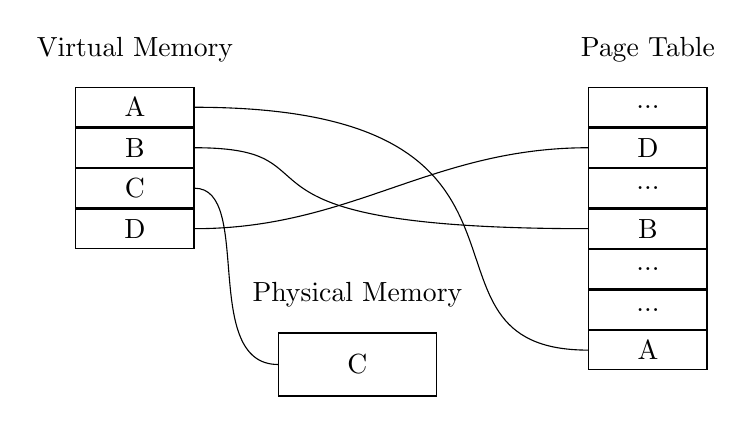
\begin{tikzpicture}[node distance=0cm]

    % Virtual Memory
    \node (vaddr1) [draw, rectangle, minimum width=1.5cm, minimum height=0.5cm] at (0,0) {A};
    \node (vaddr2) [draw, rectangle, minimum width=1.5cm, minimum height=0.5cm, below=0.0cm of vaddr1] {B};
    \node (vaddr3) [draw, rectangle, minimum width=1.5cm, minimum height=0.5cm, below=0.0cm of vaddr2] {C};
    \node (vaddr4) [draw, rectangle, minimum width=1.5cm, minimum height=0.5cm, below=0.0cm of vaddr3] {D};

    % Page Table
    \node (page1) [draw, rectangle, minimum width=1.5cm, minimum height=0.5cm, right=5cm of vaddr1] {...};
    \node (page2) [draw, rectangle, minimum width=1.5cm, minimum height=0.5cm, below=0.0cm of page1] {D};
    \node (page3) [draw, rectangle, minimum width=1.5cm, minimum height=0.5cm, below=0.0cm of page2] {...};
    \node (page4) [draw, rectangle, minimum width=1.5cm, minimum height=0.5cm, below=0.0cm of page3] {B};
    \node (page5) [draw, rectangle, minimum width=1.5cm, minimum height=0.5cm, below=0.0cm of page4] {...};
    \node (page6) [draw, rectangle, minimum width=1.5cm, minimum height=0.5cm, below=0.0cm of page5] {...};
    \node (page7) [draw, rectangle, minimum width=1.5cm, minimum height=0.5cm, below=0.0cm of page6] {A};

    % Physical Memory
    \node (paddr1) [draw, rectangle, minimum width=2cm, minimum height=0.8cm, below right=1.5cm of vaddr4] {C};
    
    % Titles
    \node[above=0.2cm of vaddr1] {Virtual Memory};
    \node[above=0.2cm of page1] {Page Table};
    \node[above=0.2cm of paddr1] {Physical Memory};
    
    % Arrows
    \draw[-] (vaddr1.east) .. controls +(right:5cm) and +(left:2.5cm) .. node[above,sloped] {} (page7.west);
    \draw[-] (vaddr2.east) .. controls +(right:2cm) and +(left:5cm) .. node[above,sloped] {} (page4.west);
    \draw[-] (vaddr3.east) .. controls +(right:0.75cm) and +(left:2cm) .. node[above,sloped] {} (paddr1);
    \draw[-] (vaddr4.east) .. controls +(right:2cm) and +(left:2cm) .. node[above,sloped] {} (page2.west);
    
    \end{tikzpicture}

    \subsubsection{Translation}
    Through the \textbf{M}emory \textbf{M}anagement \textbf{U}nit (MMU) unit and the OS it's possible to make an address translation from virtual to physical. To solve this we need to use the \textcolor{red}{\textbf{T}ranlsation \textbf{L}ookaside \textbf{B}uffer} (TLB) which is a cache for the page table
    
    \section{Optimisation}
    \begin{itemize}
        \item First rule: Set the optimisation flags, use algorithms and libraries.
        \item Second rule: Determine which part is slow. To check the time of the program, type \lstinline{time ./example}.
    \end{itemize}
    Use gprof: compile with c++ -pg main.cpp -o main, then run gprof ./main gmon.out \> prof.txt
    See week10/11 for how to use BLAS, EIGEN and LAPACK.
    \subsection{Loop unrolling}
    By extending the loop into multiple subcalculation, is possible to improve the pipelining. It's also very important to keep the \textit{static} calculations outside of the loops, such that there are no repetitions.
    

\begin{lstlisting}[language=C++, breaklines]
for(unsigned i = 0; i < N,; i += 4){
    a[i  ] = b[i  ] * c[i ];
    a[i+1] = b[i+1] * c[i+1];
    a[i+2] = b[i+2] * c[i+2];
    a[i+3] = b[i+3] * c[i+3];
}; \end{lstlisting}
    The order in which the loop is accesses matters for the speed, for example in C++
\begin{lstlisting}[language=C++, breaklines]
for(unsigned i = 0; i < N,; i += 1){
    for(unsigned j = 0; j < N,; j += 1){
        a[i][j] // Faster, row-major order
    }
}
for(unsigned j = 0; j < N,; j += 1){
    for(unsigned i = 0; i < N,; i += 1){
        a[i][j] // Slower
    }
}; 
\end{lstlisting}
    
  \subsection{Pipelining}[h]
Usually done by compiler, but can be expressed in the following way\\
but in this examples, we are adding more steps which slow down the execution.
\begin{lstlisting}[language=C++]
// Slow           // Fast
x = y;             x = y;
z = 1 + x;         z = 1 + y;\end{lstlisting}
    \subsection{Vectorisation}
    This align the memory while optimising the data dependencies and it can be achieved by adding \lstinline{-ftree-vectorize} as compile option.
    
    \subsection{Metaprograms}
    Example at \colorbox{violet!8}{\autoref{sec:meta}}.
    
    % \subsection{Lazy evaluation}
    
\subsection{Expression Templates}
\textbf{Idea 1:} We want loop unrolling when seeing an `+`. \\
\textbf{Idea 2:} We want loop unrolling even with other operators. \\
\textbf{Idea 3:} We want loop unrolling even with chains of operations. \\

\textbf{Solution 1:} Define a `vectorsum` class:
\begin{itemize}
    \item Member variables: `left` and `right`.
    \item Overload the subscript operator: `operator[](int i)` computes `left[i] + right[i]`.
    \item Overload `operator+` to return `vectorsum$<T>$(a, b)`.
    \item Overload assignment: `operator=(const vectorsum$<T>\&$ v)` with a loop: `$p\_[i]$ = v[i]`.
\end{itemize}

\textbf{Solution 2:} Generalize operations:
\begin{itemize}
    \item Introduce `operation (plus,..)` classes with member function `apply`.
    \item Replace `vectorsum` with `vectorop`, taking two template arguments.
    \item Redefine the subscript operator as: `Op::apply($left\_[i]$, $right\_[i]$)`. (assignment op stays)
    \item Overload `operator+` to return `vectorop$<T, plus>$(x, y)`.
\end{itemize}

\textbf{Solution 3:} Make operations fully general:
\begin{itemize}
    \item Replace `vectorop` with a general class `X` templated on `Left`, `Right`, and `Op`.
    \item Replace inline `vectorop$<T, plus>$ operator+` with:
    \begin{verbatim}
template<typename Left, typename T>
inline X<Left, etvector<T>, plus> operator+ (const Left& x, const etvector<T>& y);
    \end{verbatim}
    \item Redefine the assignment operator in `lazyvector` to work with `X` objects.
\end{itemize}

    \section{Python}
    Examples at \colorbox{green!7}{\autoref{sec:python}}. To search for some infos about something just type \lstinline{>>> help('print')}
    
	\begin{itemize}
	    \item Types:
        \begin{multicols}{2}
        \begin{itemize}
	       \item \textbf{Booleans}: \lstinline{True, Flase}
	       \item \textbf{Integer}: \lstinline{x = 1}
	       \item \textbf{Double}: \lstinline{x = 1.e0}
	       \item \textbf{Complex}: \lstinline{x = 1 + 1j}
	       \item \textbf{String}: \lstinline{x = "Hello! I'm a string!"}
    	\end{itemize}
        \end{multicols}
	    \item List:
        \begin{itemize}
	       \item \textbf{Insert}: \lstinline{x.insert(0,5) # Position and value}
	       \item \textbf{Remove}: \lstinline{x.pop(0) # Position}
	       \item \textbf{Value type}: \lstinline{x = [0, 1, 2, 'three'] # Arbitrary}
	       \item \textbf{Access}: \lstinline{x[-2] # Access from the right side to the left, 0 is the first position on the right}
	       \item \textbf{Adding}: \lstinline{x += [4,5,6] # [0, 1, 2, 'three', 4, 5, 6]}
	       \item \textbf{Slicing}: \lstinline{x[1:4] # [1, 2, 'three], keep only values in range 1 to 4}
	       \item \textbf{Slicing with stride}: \lstinline{x[0:7:2] == y[::2] == # [0, 2, 4, 6] (from [0, 1, 2, 'three', 4, 5, 6])}
    	\end{itemize}
	\end{itemize}
 
    \subsection{Control flow}
    \begin{itemize}
    \item if statement:
    
    \begin{lstlisting}[language=python, breaklines]
if x < 0:
    print("x is less than zero")
elif x > 0:
    print("x is greater than zero")
else:
    print("x is zero") \end{lstlisting}
    \item while loop:
    \begin{lstlisting}[language=python, breaklines]
x = 0
while x < 7:
    if x == 2:
        x += 1
        continue # skip current iteration
    if x == 6:
        break # leave loop
    print("x =",x)
    x += 1 \end{lstlisting}
    \item for loop:    
    \begin{lstlisting}[language=python, breaklines]
for i in range(5):    for letter in "String":
    print(i)             print(letter) \end{lstlisting}
    \end{itemize}
	
    \subsection{Functions}
    \begin{lstlisting}[language=python, breaklines]
def func(a, b=2, c="default"):
    ...
    return ...
func(4) # 4 2 default
func(4, 5) # 4 5 default
func(4, 5, "non-default") # 4 5 non-default\end{lstlisting}

    \subsubsection{Lambda function}
    \begin{lstlisting}[language=python, breaklines, emph={lambda}, emphstyle={\color{red}}]
def apply(func, x:
    return func(x)
x = apply(lambda z: z**2,2.)\end{lstlisting}
    \begin{lstlisting}[language=python, breaklines, emph={lambda}, emphstyle={\color{red}}]
F = lambda a,b: a-b # shortcut \end{lstlisting}
    
    \subsubsection{Pass function by argument}
    Usually functions pass by value (won't change the variables given), especially in case of simple variables like \lstinline{int, double, float} etc.
    \subsubsection{Pass function by assignment}
    In case we pass an array and modify the first value, it's possible that the returned array in \lstinline{main} results modified too. This is because the object modified in the array, corresponds to one already in use in the same array an doesn't get garbage collected:

    \begin{multicols}{2}
    \begin{lstlisting}[language=python, breaklines]
def incr(x):
    x[0] += 1
x = [0,1,2]
incr(x) # [1,1,2] \end{lstlisting}    
    \end{multicols}
    
    \subsection{Classes}
    Classes need a first argument defined by convention as \lstinline{self}, which is similar to \lstinline{this} and it's necessary to save the arguments in the class. Members can also be added automatically without having to modify the structure of the class.
\begin{lstlisting}[language=python, breaklines]
class Point:
    def __init__(self,x,y):
        self.x = x
        self.y = y
    # For normal functions, we don't use underscores
    def scale(self, sx=1,sy=1)
        self._x *= sx # To call x,y for init
        self._y *= sy # we need to set _
# To create a class
p1 = Point(0,0)\end{lstlisting}
    Some important operations are: 
    \begin{multicols}{2}
        \begin{itemize}
        \item \lstinline{__init__}: constructor
        \item \lstinline{__del__}: destructor
        \item \lstinline{__add__}: operator+
        \item \lstinline{__truediv__}: operator/
        \end{itemize}
    \end{multicols}

    
    
    \subsection{Private}
    Just set a underscore before the actual variable that must be set private as \lstinline{_private}.
    
    \subsection{Inheritance}
    We simply need to use the naming \lstinline{super())} to deal with anything regarding the parts inherited from the main class. Follows:
    
    \begin{lstlisting}[language=python, breaklines]
class A:                class B(A):
    def __init__(self):    def __init__(self):
        self.a = 1         super().__init__()
                           self.b = 2 \end{lstlisting}
    
    % \subsection{Decorators}
    
    % \subsection{Modules}
    % This is a set of functions just like in fortran.    

    \subsubsection{Import from other files}
    To import a function from another file, there are two methods:
    
    \begin{lstlisting}[language=python, breaklines]
import hello
from include.world import world # include is a folder with a file world.py in it

hello.hello() # hello is a function in a file called hello.py
world() # here we don't need to specify the folder \end{lstlisting}

    For more informations, check the code in \lstinline{ex12/solutions/pypenna}.
    
    \subsection{LinAlg}
    \subsubsection{NumPy}
    An array can be created as \lstinline{a = np.array([[1,2,3][4,5,6,...]]} and it can return / modify it's attribute with
    \begin{multicols}{2}
        \begin{itemize}
            \item \lstinline{.ndim}: dimension's array
            \item \lstinline{.shape}: tuple indicating size of array at every dimension
            \item \lstinline{.size}: number of elements
            \item \lstinline{.dtype}: returns the type of the elements in the array
        \end{itemize}
    \end{multicols}
    
    or in the other following ways:
\begin{lstlisting}[language=python, breaklines]
a = np.arange([start,] stop[, step, ])

# Linear / logarithmic 
a = np.linspace(start, stop, num) 
a = np.logspace(start, stop, num)

# Zeros / Ones matrix
a = np.zeros(shape)
a = np.ones(shape) \end{lstlisting}

    The operations are between arrays / matrices can be set with the basic math operators like \lstinline{+,-,*,/} and the slicing is the same as the standard python.
    
    \subsubsection{Matrix 2-D slicing}
    In case we have a simple 2-D matrix for plotting, we can set the X,Y axis in the following way \lstinline{X = data[:,0],Y = data[:,1]}. The first \lstinline{:} indicates that all the elements in the first column must be preserved, \lstinline{i} indicates which column to export in data.

    \subsubsection{Important notes}
    \begin{itemize}
        \item create a simple copy of an array, is like an alias. To create an indepentent copy, use \lstinline{np.copy}
        \item when trying to change the values of an array passed in a function, the values remain the same as before the call.
    \end{itemize}
    
    \subsection{Plotting}
    \subsubsection{Quick start}
        \begin{lstlisting}[language=python, breaklines]
import numpy as np
import matplotlib.pyplot as plt

X = np.linspace(0, 2*np.pi, 100)
Y = np.cos(X)
fig, ax = plt.subplots()
ax.set_title("cos(x)")
ax.legend(loc='best')
ax.plot(X, Y, color='blue'
fig.savefig("figure.pdf")
plt.show()\end{lstlisting}

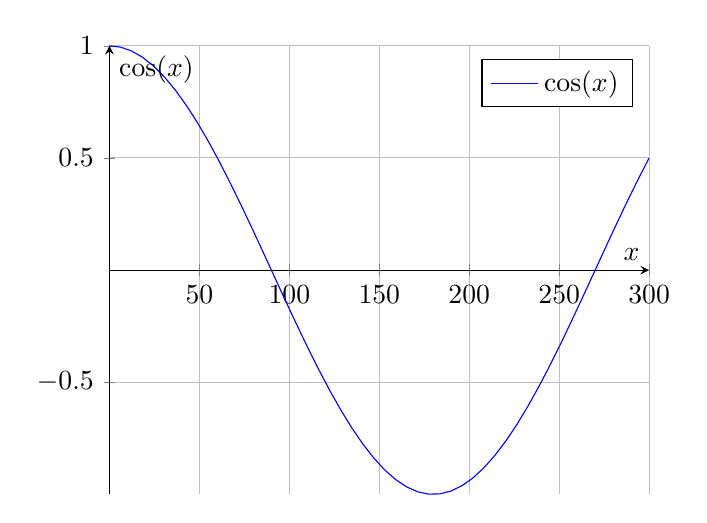
\begin{tikzpicture}
  \begin{axis}[
    xlabel={$x$},
    ylabel={$\cos(x)$},
    domain=0:300,
    samples=50,
    grid=both,
    axis lines=middle,
    legend pos=north east,
  ]
  \addplot[blue,mark=none] {cos(x)};
  \legend{$\cos(x)$}
  \end{axis}
\end{tikzpicture}

    \subsubsection{Import data}
    To import data, it's possible to use the command \lstinline{data = np.loadtxt('./result.txt').}
    
    \subsection{Plot commands}
    \begin{itemize}
        \item \lstinline{plot([X],Y,[fmt],...)}: X, Y, fmt, color, marker, linestyle 
        \item \lstinline{scatter(X,Y,...)}: X, Y, [s]izes, [c]olors, marker, cmap
        \item \lstinline{bar[h](x,height,...)}: x, height, width, bottom, align, color
        \item \lstinline{contour[f]([X],[Y],Z,...)}: X, Y, Z, levels, colors, extent, origin
        \item \lstinline{fill[_between][x](...)}: X, Y1, Y2, color, where
        \item \lstinline{step(X,Y,[fmt],...)}: X, Y, fmt, color, marker, where
    \end{itemize}
    
    \subsection{Ornaments}
    \begin{itemize}
        \item \lstinline{ax.legend(...)}: handles, labels, loc, title, frameon 
        \item \lstinline{fig.colorbar(...)}: mappable, ax, cax, orientation

    \end{itemize}
    
    \section{I/O}
    \subsection{Redirecting output}
    To redirect an output, there are 3 methods:
    \begin{itemize}
        \item \lstinline{./prog > out.dat} : output data in only a file
        \item \lstinline{./prog 1> out.dat 2> err.log} : outputs data in one file and errors in another
        \item \lstinline{./prog &> out.dat} : data and errors are in only one file
    \end{itemize}
    
    % \subsection{Formatting}
    % TO SEE LECTURE, WRITE LATER HERE
    
    \subsection{File stream}
    These are some system flags needed for \lstinline{<fstream>:}
    \begin{multicols}{2}
    \begin{itemize}
        \item \lstinline{fstream::in}
        \item \lstinline{fstream::out}
        \item \lstinline{fstream::binary}
        \item \lstinline{fstream::ate}: output starts at end
        \item \lstinline{fstream::app}: append
        \item \lstinline{fstream::trunc}: truncate
    \end{itemize}
    \end{multicols}
    
    \section{Basics}

\begin{itemize}
    \item \textbf{De-referencing:} \texttt{*x}
    \begin{itemize}
        \item Means: The object pointed to by \texttt{x}.
    \end{itemize}
    
    \item \textbf{Address-of:} \texttt{\&x}
    \begin{itemize}
        \item Means: The address of object \texttt{x}.
    \end{itemize}
    
    \item \textbf{Member of object:} \texttt{x.y}
    \begin{itemize}
        \item Means: The member \texttt{y} of object \texttt{x}.
    \end{itemize}
    
    \item \textbf{Member of pointer:} \texttt{x->y}
    \begin{itemize}
        \item Means: The member \texttt{y} of the object pointed to by \texttt{x}.
    \end{itemize}
    
    \item \textbf{Member of pointer (dereference):} \texttt{(*x).y}
    \begin{itemize}
        \item Means: The member \texttt{y} of the object pointed to by \texttt{x} (same as \texttt{x->y}).
    \end{itemize}
    
    \item \textbf{Subscript:} \texttt{x[0]}
    \begin{itemize}
        \item Means: The first object pointed to by \texttt{x}.
    \end{itemize}
    
    \item \textbf{Reference:} \texttt{Trafficlight\& f = a}
    \begin{itemize}
        \item Means: \texttt{f} becomes an alias for \texttt{a}. No copy is made, and no destructor is called for the reference.
    \end{itemize}
    
    \item \textbf{Const qualifier:} \texttt{const int\& r}
    \begin{itemize}
        \item Means: \texttt{r} is a reference to a constant integer. The value cannot be modified via \texttt{r}.
    \end{itemize}
    
    \item \textbf{Pointer arithmetic:} \texttt{p++}
    \begin{itemize}
        \item Means: Advances the pointer \texttt{p} to the next memory location.
    \end{itemize}
    
    \item \textbf{Void pointer:} \texttt{void* p}
    \begin{itemize}
        \item Means: \texttt{p} is a pointer that can store the address of any type.
    \end{itemize}
    
    \item \textbf{Null pointer:} \texttt{nullptr}
    \begin{itemize}
        \item Means: A special value indicating that a pointer is not assigned.
    \end{itemize}
\item \textbf{new} \texttt{new}
\begin{itemize}
    \item The `new` operator returns a pointer to a newly allocated object or array on the heap. For dynamic arrays (e.g., `new Type[size]`), the size can be determined at runtime or compile-time, but the memory is always allocated on the heap.
\end{itemize}
    \item \textbf{Fkt. pointer}
    \begin{itemize}
        \item Function pointer are initialized by: double (*f)(double)
    \end{itemize}
    \item \textbf{Type safety}
    \begin{itemize}
        \item function like std::printf are not typesafe as smth like printf($\%d$ 3.14) would crash at runtime as it expects an int (type correctness is not inforced by compiler)
    \end{itemize}
\end{itemize}
\section{Vim for C++ Development}

\textbf{:set mouse=a} to allow using the mouse in the terminal.

\textbf{:syntax on} to enable syntax highlighting.

\textbf{:set number} to show line numbers.

\textbf{:set autoindent} to enable automatic indentation.

\textbf{:set cindent} to enable C-style indentation.

\textbf{:set tabstop=4} to set the number of spaces for a tab (useful for aligning C++ code).

\textbf{:set shiftwidth=4} to set the number of spaces for indentation.

\textbf{:set expandtab} to convert tabs to spaces.

\textbf{gd} to go to the declaration of a variable or function under the cursor.

\textbf{K} to open the manual page for the word under the cursor (if available).

\textbf{:make} to run the build system (if configured with Makefile or \textbf{cmake}).

\textbf{:!g++ -o output file.cpp} to compile the current C++ file directly from Vim.

\textbf{:!./output} to run the compiled program.

\textbf{Ctrl + o} to jump back to the previous location.

\textbf{Ctrl + i} to jump forward to the next location.

\textbf{:vsplit file.cpp} to open another C++ file in a vertical split.

\textbf{:split file.cpp} to open another C++ file in a horizontal split.

\textbf{Ctrl + ww} to switch between split windows.

\textbf{/search\_term} to search for a specific term in the C++ code.

\textbf{n} to jump to the next occurrence of the searched term.

\textbf{N} to jump to the previous occurrence of the searched term.

\textbf{:grep search\_term \*.cpp} to search for a term across multiple C++ files.
    
    \pagebreak

\end{multicols*}

\begin{multicols*}{2}[\raggedcolumns]

\section{Examples}

\subsection{Makefile}\label{sec:makefile}
%%%%%%%%%%%%%%%%%%%%%%%%%
%This generates an error%
%%%%%%%%%%%%%%%%%%%%%%%%%
\subsubsection{General makefile}
\begin{tcolorbox}[
  %enhanced, % Allows for better line breaking
  colback=blue!7, % Background color
  colframe=blue!7, % Frame color
  boxrule=0pt, % Frame thickness
  arc=5pt, % No rounded corners
  breakable, % Allows the box to break across pages/columns
  boxsep=0pt, % Padding inside the box
  left=0pt, % Left margin
  right=0pt, % Right margin
  top=0pt, % Top margin
  bottom=0pt, % Bottom margin
  lefttitle=0pt, % Left margin for title (if you have one)
  righttitle=0pt, % Right margin for title (if you have one
]
\inputminted{makefile}{Codes/Makefile.txt}
\end{tcolorbox}

\subsubsection{Library creation with Make}
\begin{tcolorbox}[
  %enhanced, % Allows for better line breaking
  colback=blue!7, % Background color
  colframe=blue!7, % Frame color
  boxrule=0pt, % Frame thickness
  arc=5pt, % No rounded corners
  breakable, % Allows the box to break across pages/columns
  boxsep=0pt, % Padding inside the box
  left=0pt, % Left margin
  right=0pt, % Right margin
  top=0pt, % Top margin
  bottom=0pt, % Bottom margin
  lefttitle=0pt, % Left margin for title (if you have one)
  righttitle=0pt, % Right margin for title (if you have one
]
\inputminted{makefile}{Codes/Makefile_library.txt}
\end{tcolorbox}

\subsection{CMake}\label{sec:cmake}
\subsubsection{Main}
\begin{tcolorbox}[
  %enhanced, % Allows for better line breaking
  colback=red!7, % Background color
  colframe=red!7, % Frame color
  boxrule=0pt, % Frame thickness
  arc=5pt, % No rounded corners
  breakable, % Allows the box to break across pages/columns
  boxsep=0pt, % Padding inside the box
  left=0pt, % Left margin
  right=0pt, % Right margin
  top=0pt, % Top margin
  bottom=0pt, % Bottom margin
  lefttitle=0pt, % Left margin for title (if you have one)
  righttitle=0pt, % Right margin for title (if you have one
]
\inputminted{cmake}{Codes/CMakeLists.txt}
\end{tcolorbox}



\subsubsection{Libraries}
\begin{tcolorbox}[
  %enhanced, % Allows for better line breaking
  colback=red!7, % Background color
  colframe=red!7, % Frame color
  boxrule=0pt, % Frame thickness
  arc=5pt, % No rounded corners
  breakable, % Allows the box to break across pages/columns
  boxsep=0pt, % Padding inside the box
  left=0pt, % Left margin
  right=0pt, % Right margin
  top=0pt, % Top margin
  bottom=0pt, % Bottom margin
  lefttitle=0pt, % Left margin for title (if you have one)
  righttitle=0pt, % Right margin for title (if you have one
]
\inputminted{cmake}{Codes/CMakeLists_libraries.txt}
\end{tcolorbox}



\subsubsection{Tests}
\begin{tcolorbox}[
  %enhanced, % Allows for better line breaking
  colback=red!7, % Background color
  colframe=red!7, % Frame color
  boxrule=0pt, % Frame thickness
  arc=5pt, % No rounded corners
  breakable, % Allows the box to break across pages/columns
  boxsep=0pt, % Padding inside the box
  left=0pt, % Left margin
  right=0pt, % Right margin
  top=0pt, % Top margin
  bottom=0pt, % Bottom margin
  lefttitle=0pt, % Left margin for title (if you have one)
  righttitle=0pt, % Right margin for title (if you have one
]
\inputminted{cmake}{Codes/CMakeLists_test.txt}
\end{tcolorbox}

\begin{tcolorbox}[
  %enhanced, % Allows for better line breaking
  colback=red!7, % Background color
  colframe=red!7, % Frame color
  boxrule=0pt, % Frame thickness
  arc=5pt, % No rounded corners
  breakable, % Allows the box to break across pages/columns
  boxsep=0pt, % Padding inside the box
  left=0pt, % Left margin
  right=0pt, % Right margin
  top=0pt, % Top margin
  bottom=0pt, % Bottom margin
  lefttitle=0pt, % Left margin for title (if you have one)
  righttitle=0pt, % Right margin for title (if you have one
]
\inputminted{cmake}{Codes/CMakeLists_test_folder.txt}
\end{tcolorbox}

\subsection{Type traits}\label{sec:traits} 
\begin{tcolorbox}[
  %enhanced, % Allows for better line breaking
  colback=orange!7, % Background color
  colframe=orange!7, % Frame color
  boxrule=0pt, % Frame thickness
  arc=5pt, % No rounded corners
  breakable, % Allows the box to break across pages/columns
  boxsep=0pt, % Padding inside the box
  left=0pt, % Left margin
  right=0pt, % Right margin
  top=0pt, % Top margin
  bottom=0pt, % Bottom margin
  lefttitle=0pt, % Left margin for title (if you have one)
  righttitle=0pt, % Right margin for title (if you have one
]
\inputminted{C++}{Codes/Traits.txt}
\end{tcolorbox}



\subsection{Exceptions}\label{sec:exceptions}
\begin{tcolorbox}[
  %enhanced, % Allows for better line breaking
  colback=purple!7, % Background color
  colframe=purple!7, % Frame color
  boxrule=0pt, % Frame thickness
  arc=5pt, % No rounded corners
  breakable, % Allows the box to break across pages/columns
  boxsep=0pt, % Padding inside the box
  left=0pt, % Left margin
  right=0pt, % Right margin
  top=0pt, % Top margin
  bottom=0pt, % Bottom margin
  lefttitle=0pt, % Left margin for title (if you have one)
  righttitle=0pt, % Right margin for title (if you have one
]
\inputminted{C++}{Codes/Exceptions.txt}
\end{tcolorbox}



\subsection{Testing}\label{sec:test}
\subsubsection{CMakeLists - test folder}
\begin{tcolorbox}[
  %enhanced, % Allows for better line breaking
  colback=yellow!7, % Background color
  colframe=yellow!7, % Frame color
  boxrule=0pt, % Frame thickness
  arc=5pt, % No rounded corners
  breakable, % Allows the box to break across pages/columns
  boxsep=0pt, % Padding inside the box
  left=0pt, % Left margin
  right=0pt, % Right margin
  top=0pt, % Top margin
  bottom=0pt, % Bottom margin
  lefttitle=0pt, % Left margin for title (if you have one)
  righttitle=0pt, % Right margin for title (if you have one
]
\inputminted{cmake}{Codes/CMakeLists_test_folder.txt}
\end{tcolorbox}

\subsubsection{Code}
\begin{tcolorbox}[
  %enhanced, % Allows for better line breaking
  colback=yellow!7, % Background color
  colframe=yellow!7, % Frame color
  boxrule=0pt, % Frame thickness
  arc=5pt, % No rounded corners
  breakable, % Allows the box to break across pages/columns
  boxsep=0pt, % Padding inside the box
  left=0pt, % Left margin
  right=0pt, % Right margin
  top=0pt, % Top margin
  bottom=0pt, % Bottom margin
  lefttitle=0pt, % Left margin for title (if you have one)
  righttitle=0pt, % Right margin for title (if you have one
]
\inputminted{C++}{Codes/Test.txt}
\end{tcolorbox}

\subsection{Optimisation}
\subsubsection{Meta-programming}\label{sec:meta}
\begin{tcolorbox}[
  %enhanced, % Allows for better line breaking
  colback=violet!8, % Background color
  colframe=violet!8, % Frame color
  boxrule=0pt, % Frame thickness
  arc=5pt, % No rounded corners
  breakable, % Allows the box to break across pages/columns
  boxsep=0pt, % Padding inside the box
  left=0pt, % Left margin
  right=0pt, % Right margin
  top=0pt, % Top margin
  bottom=0pt, % Bottom margin
  lefttitle=0pt, % Left margin for title (if you have one)
  righttitle=0pt, % Right margin for title (if you have one
]
\inputminted{C++}{Codes/Metaprogramming.txt}
\end{tcolorbox}

\begin{tcolorbox}[
  %enhanced, % Allows for better line breaking
  colback=violet!8, % Background color
  colframe=violet!8, % Frame color
  boxrule=0pt, % Frame thickness
  arc=5pt, % No rounded corners
  breakable, % Allows the box to break across pages/columns
  boxsep=0pt, % Padding inside the box
  left=0pt, % Left margin
  right=0pt, % Right margin
  top=0pt, % Top margin
  bottom=0pt, % Bottom margin
  lefttitle=0pt, % Left margin for title (if you have one)
  righttitle=0pt, % Right margin for title (if you have one
]
\inputminted{C++}{Codes/MetaprogrammingLoop.txt}
\end{tcolorbox}

\subsection{Python}\label{sec:python}
\subsubsection{Classes}
\begin{tcolorbox}[
  %enhanced, % Allows for better line breaking
  colback=green!7, % Background color
  colframe=green!7, % Frame color
  boxrule=0pt, % Frame thickness
  arc=5pt, % No rounded corners
  breakable, % Allows the box to break across pages/columns
  boxsep=0pt, % Padding inside the box
  left=0pt, % Left margin
  right=0pt, % Right margin
  top=0pt, % Top margin
  bottom=0pt, % Bottom margin
  lefttitle=0pt, % Left margin for title (if you have one)
  righttitle=0pt, % Right margin for title (if you have one
]
\inputminted{python}{Codes/Python_classes.txt}
\end{tcolorbox}
\subsubsection{LinAlg}
\begin{tcolorbox}[
  %enhanced, % Allows for better line breaking
  colback=green!7, % Background color
  colframe=green!7, % Frame color
  boxrule=0pt, % Frame thickness
  arc=5pt, % No rounded corners
  breakable, % Allows the box to break across pages/columns
  boxsep=0pt, % Padding inside the box
  left=0pt, % Left margin
  right=0pt, % Right margin
  retutop=0pt, % Top margin
  bottom=0pt, % Bottom margin
  lefttitle=0pt, % Left margin for title (if you have one)
  righttitle=0pt, % Right margin for title (if you have one
]
\inputminted{python}{Codes/simple_plot.txt}
\end{tcolorbox}
\begin{tcolorbox}[
  %enhanced, % Allows for better line breaking
  colback=green!7, % Background color
  colframe=green!7, % Frame color
  boxrule=0pt, % Frame thickness
  arc=5pt, % No rounded corners
  breakable, % Allows the box to break across pages/columns
  boxsep=0pt, % Padding inside the box
  left=0pt, % Left margin
  right=0pt, % Right margin
  top=0pt, % Top margin
  bottom=0pt, % Bottom margin
  lefttitle=0pt, % Left margin for title (if you have one)
  righttitle=0pt, % Right margin for title (if you have one
]
\inputminted{Python}{Codes/Python_linalg.txt}
\end{tcolorbox}


\subsubsection{Plotting}
\begin{tcolorbox}[
  %enhanced, % Allows for better line breaking
  colback=green!7, % Background color
  colframe=green!7, % Frame color
  boxrule=0pt, % Frame thickness
  arc=5pt, % No rounded corners
  breakable, % Allows the box to break across pages/columns
  boxsep=0pt, % Padding inside the box
  left=0pt, % Left margin
  right=0pt, % Right margin
  top=0pt, % Top margin
  bottom=0pt, % Bottom margin
  lefttitle=0pt, % Left margin for title (if you have one)
  righttitle=0pt, % Right margin for title (if you have one
]
\inputminted{python}{Codes/Python_plotting.txt}
\end{tcolorbox}



    \textbf{Tipps:}
    \begin{itemize}
        \item The preprocessor can enable computation of parts of the source code
        \item The order in which the linker combines the libraries into an executable is important
        \item A program must always contain main
        \item Object files don't contain readable instructions
        \item Function templates can only be fully specialised
        \item Polynomial computational time can be achieved with function overloading
        \item Template instatiation always occurs at compile time
        \item Polynomial runtime can be achieved with virtual functions
        \item After \textbf{catch} there can be a \textbf{try} statement
        \item Executables do not need to have the preprocessor DEBUG defined
        \item An uncaught exception leads to a crash in the program
        \item If elements on a large array are read only once, the order does affect the cache hit-rate
        \item The memory is being outperformed by the CPU speed
        \item Assembly code is \textbf{by no mean} portable
        \item S(tatic)RAM is faster than D(ynamic)RAM
    \end{itemize}
\end{multicols*}
\end{document}